
% The default theme, with plain white background
\documentclass{smilebeamer}

% If you don't like oranges and such in the background remove the [bgimages] like this :
% \documentclass{smilebeamer}

\usepackage[francais]{babel}
\usepackage[utf8]{inputenc}
\usepackage{eurosym}
\usepackage{hyperref}
\usepackage{minted}



\renewcommand{\familydefault}{\sfdefault}
\usepackage{helvet}
%\usepackage{avant}
\usepackage[T1]{fontenc}


%\usebackgroundtemplate
%{
%    \includegraphics[width=\paperwidth,height=\paperheight]{img/bg.jpg}
%}


\title{Réseaux de capteurs OpenSource}
\author{Nicolas Aguirre}

\begin{document}

%%%%%%%%%%%%%%%%%%%%%%%%%%%%%
\begin{frame}[plain]
  \title{Réseaux de capteurs OpenSource}
    \titlepage
\end{frame}

\section{Moi}

% Passion == Capteurs de températures
% Réchauffement climatique ?
% Bien être personnel ?
% Tromatisme des le plus jeune age ?


\begin{frame}
\frametitle{Moi}
\begin{center}
Ma grande passion les capteurs de températures !
\newline 
(je peux en parler pendant des heures, et je suis libre le Mercredi soir)
\end{center}


\end{frame}

\begin{frame}
\frametitle{Moi}
J'aime bien aussi les petits machins :

\begin{itemize}
\item Quand ca tient dans la main
\item Que ca s'alimente sur pile bouton pendants des années
\item Qu'il y a pas beaucoup de flash et de ram
\end{itemize}
\end{frame}

\begin{frame}
\frametitle{Moi}
\begin{center}
J'aime pas les fils.
\end{center}
\end{frame}

\begin{frame}
\frametitle{Moi}
Mais je ne suis pas Masochiste.
\begin{itemize}
\item Donc j'aime pas (trop) l'assembleur
\item Et je préfére le C
\end{itemize}
\end{frame}

\begin{frame}
\frametitle{Moi}
J'aime bien quand toutes les machines causent entre elles et que même ca s'apelle l'internet.
\end{frame}


{
\usebackgroundtemplate{\includegraphics[width=\paperwidth]{img/placement_produit.jpg}}%
\begin{frame}
\end{frame}
}

\begin{frame}
\frametitle{Moi}

\begin{center}
\includegraphics{img/calaos_about_logo.png}
\newline
J'aime la domotique et surtout le projet Calaos. (GPLv3!)
\end{center}
\end{frame}

\begin{frame}
\frametitle{Moi}
\begin{center}
J'aime beaucoup les normes et des RFC
\newline 
(mais j'aime pas les lire)
\end{center}
\end{frame}

\begin{frame}
\frametitle{Moi}
\begin{center}
J'aime l'IoT (celui des hipies pas celui des hipsters)
\end{center}

J'aime les objets communicants que l'on a commencé à développer dans
les années 70 et qui, encore aujourd'hui continuent de communiquer
ensemble.
\end{frame}


\begin{frame}
\frametitle{Moi}
\begin{center}
Et ... Je suis Fan de logiciel libre !
\end{center}
\end{frame}

\begin{frame}
\frametitle{Moi}
\begin{center}
Pour toutes ces raisons, j'ai commencé à m'intéresser aux capteurs de réseaux sans fil.
\end{center}
\end{frame}

\begin{frame}
\frametitle{Mais quelles techno pour les réseaux sans fil ?}

% Zigbee proprio
% Zwave prorpio, OpenZwave ouverture des protocoles ca va dans le bon sens
% 433/868Mhz interressant, mais pas sécurisé, pas de mesh, sympa pour piloter des prises
% Mysensors et NRF24L01 : interessant, mais pas toujours tres fiable.
% EnOcean, techno génial : pas de fil, pas de pile, utilise la collecte d'energie mais pas ou peu sécurisé (derniere version de la norme mieux ?)
% Threads : Norme / Consortium avec des grands de l'industrie, a fait un flop et puis OpenThreads : implémentation open source, mais pas de version pour des microcontroleurs
% 6LowPan : le champ' IPv6, mesh, RFC, implémentation sur différents OS opensource dont Linux !

\begin{itemize}
\item Zigbee
\item Zwave
\item 433Mhz / 868Mhz
\item NRF24L01
\item EnOcean
\item Threads
\item 6LowPan
\end{itemize}
\end{frame}

\section{6LowPan}

\begin{frame}
\frametitle{6LowPAN}
\begin{itemize}
\item 6LowPAN =  IPv6 LoW Power wireless Area Networks
\item C'est le nom d'un groupe de travail de l'IETF
\item basé sur le compression d'entête de paquets IPv6
\item Par ce biais permet a ces paquets de transiter sur des réseaux sans fil de type 802.15.4
\item 802.15.4 : payload de 128Bytes
\item alors qu'IPv6 impose une MTU minimal de 1280 Bytes
\end{itemize}
\end{frame}

\begin{frame}
\frametitle{RFC 6LowPAN} 
\begin{itemize}
\item la RFC4919 https://tools.ietf.org/html/rfc4919: IPv6 over Low-Power Wireless Personal Area Networks (6LoWPANs)
\item ma RFC4944 https://tools.ietf.org/html/rfc4944 :  Transmission of IPv6 Packets over IEEE 802.15.4 Networks
\end{itemize}
\end{frame}

\begin{frame}
\frametitle{Un mot sur Ipv6}

On est en rupture d'adresses IPv4 (il se dit que ...)
\newline 
\begin{itemize}
\item $2^{32}$ = 4294967296 adresses possibles
\item $2^{128}$ = Brain overflow
\end{itemize}
 
Passons donc à IPv6 c'est trop stylé (dixit les stagiaires) et puis on
a pas trop le choix, c'est les fondements de 6LowPAN.

\end{frame}

\begin{frame}
\frametitle{Un mot sur Ipv6}

Il faudrait 667 millions de millards d'appareils connectés par millimètres carrés pour épuiser le stock d'adresse IP.

\end{frame}


\begin{frame}
\frametitle{Exercice}
\begin{itemize}
\item Connaissant le nombre d'appareils connectés par millimètres carrés
\item Qu'un appareil consomme en moyenne 100uA sous 3v
\item Quelle est la puissance nécessaire pour alimenter les objets connectés sur la superficie de la France ?
\end{itemize}
\end{frame}

\begin{frame}
\frametitle{Exercice}

Quelqu'un ?

\end{frame}

\begin{frame}[fragile]

\frametitle{16 mots sur l'IPv6}

\begin{itemize}
\item Les adresses sont l:oo:oo:oo:oo:oo:oo:oo:oo:gues
\item Et donc difficiles a retenir et en hexadécimal.
\item Mais elles peuvent être affichées compressées;
\item La règle est : on peut supprimer une fois dans une adresse une série de 0 et remplacer ça par ":"
\item Donc par exemple, l'adresse suivante : 


\begin{consolecode}
F00D:0000:0000:0000:0000:0000:DEAD:BEEF
\end{consolecode}

\item peut s'écrire : 
\begin{consolecode}
F00D::DEAD:BEEF
\end{consolecode}
\end{itemize}
\end{frame}


\begin{frame}
\frametitle{Abondance d'IPs ne nuit pas}

Mais change la philosophie :
\begin{itemize}

\item Les interfaces réseaux peuvent avoir plusieurs adresses IP.
\begin{itemize}
\item Une adresse lien-locale obligatoire (limité au lien L2, i.e
Ethernet) et commencent par FE80
\item Une ou plusieurs autres adresses données par un DHCPv6 ou calculé a partir d'un Prefix et de l'adresse MAC
\end{itemize}

\item L'implémentation du multicast est obligatoire
\item Le broadcast est remplacé par le multicast sur le lien locale
\item Le multicast est la base du protocole ND (remplacement d'ARP)
\item Il n'y a plus de protocoles à cheval entre L2 et L3 (ARP, DHCP)
\end{itemize}

\end{frame}

\begin{frame}
\frametitle {802.15.4}

Protocole de communication IEEE pour les réseau sans fil
Fait pour les LR WPAN : Low Rate Wireless Personnal Area Network)
\begin{itemize}
\item Faible consommation
\item Faible débit
\item Faible portée
\end{itemize}
Utilisé dans différentes implémentations :
\begin{itemize}
\item IP : 6LowPan
\item Propriétaire : Zigbee
\end{itemize}
\end{frame}

\begin{frame}
\frametitle {802.15.4}
\begin{itemize}
\item Permet les réseau de type Etoile ou Mesh
\item Adresses sur 16 ou 64 bits
\item Méthode d'accès au media CSMA/CA (identique au wifi)
\item Faible Consommation d'énergie
\item Indication sur la qualité de liaison LQI
\item Différentes Bande de fréquences possible :
\begin{itemize}
  \item  16 Canaux de 2.4 a 2.4835 GHz
  \item  10 canaux de 902 a 928 MHz (US)
  \item 1 Canal dans la bande 868 a 868.6 MHz (EU)
\end{itemize}
  \end{itemize}
\end{frame}

\begin{frame}

\frametitle{6LowPan}
\begin{itemize}
\item LowPan est un réseau contraint en ressources (faible CPU, mémoire et batterie)
\item Le débit du réseau est limité (jusqu'a 250Kb/s)
\item La MTU d'un réseau 802.15.4 est de 128Bytes
\item L'entête de la couche MAC est de 25Bytes
\item => il ne reste que 102 bytes pour les couches supérieur
\item La couche de sécurisation des données AES ajoute 21 Bytes supplémentaires
  \end{itemize}
\end{frame}

% 6lowpan c'est cool, mais comment on le met en place ? de quoi on a besoin ?

\begin{frame}
\frametitle{Mise en place}

On a besoin de : 

\begin{itemize}
\item une machine qui émet des données 6lowpan
\item une machine qui reçoit des données IPv6
\item une machine qui sert de passerelle entre le 6lowPAN et l'IPv6
\end{itemize}
\end{frame}

\begin{frame}
\frametitle{Mise en place}
\includegraphics[width=12cm,height=7cm]{img/6lowpan.png}
\end{frame}


\begin{frame}
\frametitle{Machine émettrice}
\begin{center}
SensorTAG de Texas Instruments
\includegraphics{img/sensortag.png}


\end{center}
\end{frame}

\begin{frame}
\frametitle{Machine émettrice}
\begin{center}

\includegraphics[width=10cm,height=5cm]{img/sensortag-teardown.png}


\end{center}
\end{frame}


\begin{frame}
\frametitle{Machine réceptrice}

Un PC avec un GNU/Linux ou tout autre solution compatible IPv6


Et même IPv4

\end{frame}

\begin{frame}
\frametitle{Passerelle}

Une RaspberryPI et un SensorTAG pour le support du 802.15.4
\includegraphics[width=10cm,height=5cm]{img/border_router.jpg}
\end{frame}

\begin{frame}
\frametitle{Coût Total}
\begin{itemize}
\item Une RaspberryPI : 45 euros
\item Un SensorTAG pour le BR: 30 euros
\item Un pack debug (pour l'USB série) : 30 euros
\item Un SensorTAG : 30 euros
\item Un PC : on le compte ?
\end{itemize}
\end{frame}

\begin{frame}
\frametitle{SensorTag}
\begin{itemize}
\item Carte de dev "prête" à l’emploi développée par Texas Instrument
\item Cortex M3 48MHz 128KB de Flash 8KB de RAM
\item Flash externe de 512KB (pour mise à jour OTA ou stockage)
\item Consommation 10mA en émission, 100uA en veille
\item Radio 802.15.4 ET Bluetooth Low Energy (BLE)
\item 30 euros en quantités limitées sur le site de TI (max 3 par commandes :'( :'( :'( )
\item Fonctionnement sur pile boutons
\end{itemize}
\end{frame}

\begin{frame}
\frametitle{SensorTag}

Les SensorTAG supportent l'OS Contiki.
\newline
Génial c'est Open Source (licence BSD)

\end{frame}




\section{Contiki}


\begin{frame}
\frametitle{Multitâche coopératif}

Contiki est un système d'exploitation
\begin{itemize}
\item open source 
\item multi-tâches
\item portable
\end{itemize}

Idéal pour 
\begin{itemize}
\item les systèmes embarqués 
\item les réseaux de capteurs sans fil (WSN: Wireless sensor network) 
 \end{itemize}
 
Contiki est conçu spécifiquement pour des Micro-contrôleurs avec de petites quantités de mémoire. 
Une configuration typique :
\begin{itemize}
\item 2 Ko de RAM 
\item 40 Ko de ROM
 \end{itemize}
\end{frame}

\begin{frame}
\frametitle{Contiki}

Contiki est écrit en C et est disponible sous licence BSD.

Contiki est utilisé principalement pour son support des réseau IP :
\begin{itemize}
\item IPv4
\item IPv6
\end{itemize}

La pile uIPv6 est certifiée IPv6 Ready Phase 1 par CISCO

La pile Ip de contiki uIP a été initialement publié en 2011 et est aujourd'hui utilisée industriellement par différentes entreprises à travers le monde.

\end{frame}


\begin{frame}
\frametitle{Contiki}
Contiki est développé par une équipe de développeurs du domaine de l'industrie et du domaine universitaire. 
Le développeur principal :
\begin{itemize}
\item Adam Dunkels
\item Swedish Institute of Computer Science.
\end{itemize}
\end{frame}


\begin{frame}
\frametitle{Multitâche coopératif}
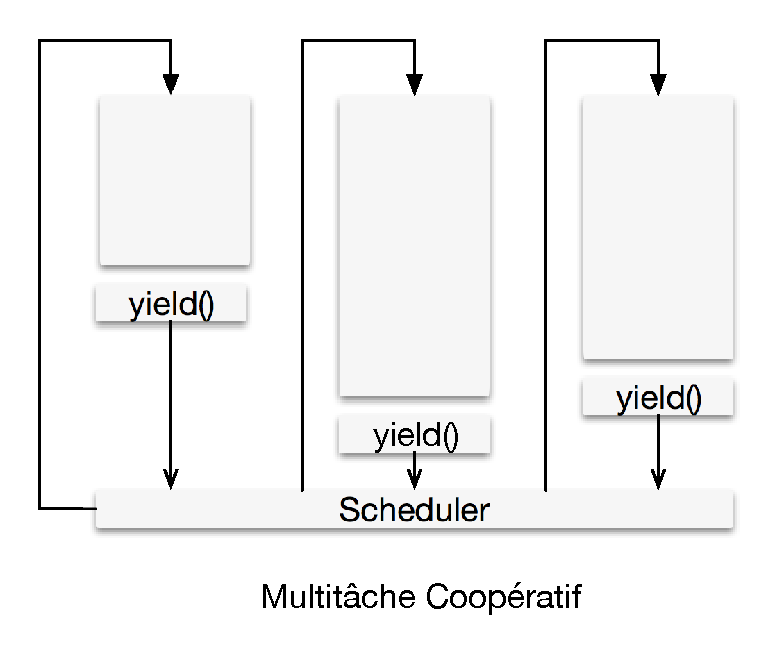
\includegraphics[width=10cm,height=8cm]{img/multitache_coop.eps}
\end{frame}


\begin{frame}

\frametitle{Proto-Threads}
\begin{itemize}
\item Spécificité de contiki.
\item Développés par Adamn Dunkels.
\item  Threads extrêmement légers et dépourvus de stack (stackless)
\item  Conçus spécifiquement pour les systèmes ultra contraints en mémoire.
\item  Fournissent une exécution de code linéaire pour les "event-driver".
\item  Sont implémentés en C.
\item Peuvent être utilisés avec ou sans un système d'exploitation sous jacent.
\item Permettent un contrôle de flux séquentiel sans avoir recours à des machine à états complexes.
\item Permettent de se passer de la lourdeur d'un système multi threads complet.
\end{itemize}
\end{frame}

%- Mais _**ne peut pas fonctionner si on est dans un seul et même thread**_.
%- Dans un système avec OS, nous utiliserions les pthreads et des primitives de synchronisation pour communiquer entre les deux fonctions.

%Les protothreads amènent ici, par l'utilisation de macros, la possibilité de faire du multithreads sans ajouter la lourdeur d'un OS.
%Uniquement en utilisant des subtilités du langage C.
\begin{frame}[containsverbatim]

\frametitle{Proto-Threads}

exemple de code :
  \begin{minted}[fontsize=\scriptsize]{C}
#include "pt.h"

static int counter;
static struct pt example_pt;

static
PT_THREAD(example(struct pt *pt))
{
  PT_BEGIN(pt);

  while(1) {
    PT_WAIT_UNTIL(pt, counter == 1000);
    printf("Seuil atteint\n");
    counter = 0;
  }

  PT_END(pt);
}
  \end{minted}
\end{frame}

\begin{frame}[containsverbatim]

\frametitle{Proto-Threads}

Et voici une version allégée de ce a quoi ressemble les MACROS :
  \begin{minted}[fontsize=\scriptsize]{C}

struct pt
{
    unsigned short lc;
};

#define PT_THREAD(name_args)  char name_args

#define PT_BEGIN(pt)          switch(pt->lc) { case 0:

#define PT_WAIT_UNTIL(pt, c)  pt->lc = __LINE__; \
	                      case __LINE__: \
                              if(!(c)) return 0
                              
#define PT_END(pt)            } pt->lc = 0; return 2

#define PT_INIT(pt)           pt->lc = 0

  \end{minted}
\end{frame}

\begin{frame}[containsverbatim]
\frametitle{Proto-Threads}

Et voici une version allégée de ce a quoi ressemble les MACROS :
  \begin{minted}[fontsize=\scriptsize]{C}

static char example(struct pt *pt)
{
  switch(pt->lc) { case 0:

  while(1) {
    pt->lc = 12; case 12:
    if(!(counter == 1000)) return 0;
    printf("Seuil atteint\n");
    counter = 0;
  }

  } pt->lc = 0; return 2;
}



  \end{minted}
\end{frame}

\begin{frame}[containsverbatim]
\frametitle{Proto-Threads}

Vous aussi vous trouvez ca SALE ?

\end{frame}


\begin{frame}[containsverbatim]
\frametitle{Proto-Threads}

Oui mais :
\begin{itemize}

\item OverHead très faible: Seulement 2 octets par protothreads et pas de RAM dédié a la pile.
\item Code portable: écrit en C et aucun code écrit en assembleur.
\item Peut être utilisé avec ou sans OS
\item Fourni des attentes bloquantes sans changement de contexte
\end{itemize}
\end{frame}

\begin{frame}

Avec Contiki et un SensorTag on a la possibilité de communiquer en 6LowPan avec d'autres.

Mais on veux faire de l'IP !

Il nous faut une passerelle pour passer du 6LowPan à l'IPv6

C'est la que 6LBR entre en jeux !

\end{frame}

\section{6lbr}

\begin{frame}
\frametitle{6LBR}
Projet initié par la société Belge Cetic :  https://www.cetic.be/

6lbr est un fork de Contiki

6LBR est une solution de Routeur de Bordure 6LowPan / RPL
Il peut fonctionne en tant qu'application sur une carte embarqué ou sur un hôte Linux.
Il est conçu pour être flexible.
Il peut être configuré pour s'adapter a différente topologies réseau et interconnecter les réseaux de capteur sans fil au monde IP
\end{frame}

\begin{frame}
\frametitle{6LBR}

Le but de 6Lbr est d'interconnecter un réseau WSN basé sur le 802.15.4 et 6LowPan avec un réseau IPv6 basé sur l'Ethernet ou le Wifi.
\newline
Cette connexion peut être réalisé a différents niveaux du modèle OSI.
\begin{itemize}

\item Au niveau 2, link layer            => on parle de pont réseau (bridge) ou de switch;
\item Au niveau 3, network layer     => on parle de routeur (router)
\item Au niveau 7, application layer => on parle de passerelle (gateway)
\end{itemize}

6LBR est une plateforme prête a l'emploi pour interconnecter des réseaux 6LowPAN et des réseaux IP. Il part du principe qu'il existe une interface du côté IP et une autre de type 802.15.4 du côté 6LowPAN.
\end{frame}

\begin{frame}
\frametitle{6LBR}

Pour intégrer 6LBR sur notre RPI :
\begin{itemize}
\item Soit on prend Raspbian, et on compile en prenant les sources sur 
https://github.com/cetic/6lbr/
\item Soit on prend OpenEmbedded et on peux ajouter le layer meta-6lbr ici:
https://github.com/Openwide-Ingenierie/meta-6lbr
\end{itemize}
\end{frame}


\begin{frame}
\frametitle{6LBR}

Une fois que l'on a installé 6LBR sur la machine

\end{frame}

\section{Démo}

\begin{frame}
\frametitle{IFTTT}

IFTTT = If This Then That
\begin{itemize}
\item Webservice permettant de connecter différents services web entre eux via des actions primaires.
\item C'est assez limité, mais assez intéressant pour la démo.
\item Permet de faire des requêtes HTTP via un "Channel Maker"
Pas possible de faire du IFTATTT (If This and This Then That)
\end{itemize}
\end{frame}

\begin{frame}
\frametitle{IP64}
\begin{itemize}
\item Un problème pas d'IPv6 pour IFTTT !
\item Il faut donc passer par de l'IPv4.
\item 6LBR gère le IP64
\item On encapsule les adresses IPV4 dans des adresses IPV6.
\item Dans l'autre sens c'est du NAT 4 to 6.
\end{itemize}
\end{frame}

\begin{frame}
\frametitle{Show me the code}
\begin{center}
https://github.com/Openwide-Ingenierie/contiki-boite-a-meuh
\end{center}
\end{frame}

\end{document}
